\begin{usecase}{Schedule Prayer Times}
    \ucbasicinfo{High}{Regular}
    \ucshortdescription{The calendar is blocked and updated automatically according to the person's time zone prayer time.}
    \uctrigger{This usecase triggered when the user enables the prayer time feature in the application.}
    \ucactors{User}{None}
    \ucpreconditions{User must be logged into the system.}
    \ucrelationships{N/A}{N/A}{N/A}
    \ucinputsoutputs{
      \begin{itemize}
        \item \textbf{User's time Zone} (Source: user)
        \item \textbf{We get the IP address of the user and get their time zone}
      \end{itemize}
    }{
      \begin{itemize}
        \item \textbf{The calendar displays the blocked time for prayer time according to their time zone.}
      \end{itemize}
      }
    \ucmainflow{
      \begin{enumerate}
        \item User enables the feature by clicking the the option Schedule Prayer Time.
          \ucinfo{The system checks the time zone of the user and blocks the calendar accordingly.}
      \end{enumerate}
    }
    \ucalternateflows{
      \begin{itemize}
        \item The user doesn't enable the scheduling prayer time.
      \end{itemize}
    }
    \ucexceptions{
      \begin{itemize}
        \item If there's a system error, display a relevant error message.
      \end{itemize}
    }
    \ucpostconditions{The system generates calendar with prayer time}
    \ucspecialrequirements{The system must block the calendar according to their time zone}
    \ucconclusion{User's prayer times are successfully scheduled.}
    \ucbusinessrules{
      \begin{itemize}
        \item Prayer times must be within valid time ranges.
      \end{itemize}
    }
\end{usecase}

\begin{figure}[!h]
  \centering
  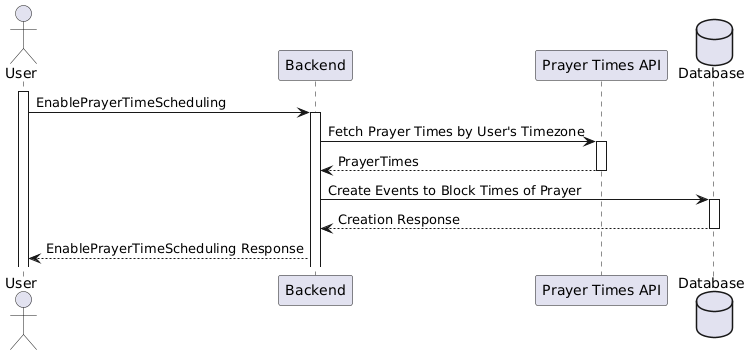
\includegraphics[width=\textwidth]{images/docs/diagrams/sequence-diagrams/all-sequence-diagrams/Schedule Prayer Times.png}
  \caption{Schedule Prayer Times Sequence Diagram}
  \label{fig:seq/schedule-prayer-times}
\end{figure}